\section{AEIC介导的Leader--Follower机制}\label{sec:game}
\subsection{时序与行动空间}
Leader在生成前承诺合同$m$，追随者观察后选择
\begin{equation}a_i\in\mathcal{A}=\{\textsc{Low},\textsc{AEIC},\textsc{Verify},\textsc{Imitate}\}.\end{equation}
四种行动分别触发低成本短报告、独立完整AEIC推理、追加验证调用和同伴信息综合。行动会选择不同Prompt、Token上限，并在分层执行器中选择不同模型资源。

合同包含信用规则$g_m$、行动成本$c_m(a)$、信息策略和验证预算。追随者的净效用写为
\begin{equation}U_i(a_i;m,h_i)=\mathbb{E}[g_m(r_i,y,h_i)\mid a_i,m,h_i]-c_m(a_i),\label{eq:followerutility}\end{equation}
其中$h_i$为可见历史，$y$仅在需要结果验证时对结算环境可用。本文不声称模型精确计算该式；检验对象是奖励或成本变化时行动分布是否改变。

\subsection{比较规则}
确认性实验固定问题、Seed、面板、轮数和信息策略，比较No Mechanism、Outcome Only和Static AEIC。前者不提供显式信用；第二种仅为正确最终立场结算；第三种按AEIC完整性和合法结论结算且不读取答案键。令$H(a)=\mathbf{1}[a\in\{\textsc{AEIC},\textsc{Verify}\}]$。主要估计量分别是$\mathbb{E}[H]$和问题级多数票正确率的配对变化，Token作为资源结果单独报告。

\subsection{结算与纵向状态}
\begin{equation}\rho_i^t=\delta\rho_i^{t-1}+g_m(r_i^t,y,h_i^t)-c_m(a_i^t),\qquad\delta=0.9.\end{equation}
静态规则不按信誉自适应系数，但保留完整状态以支持历史消融与未来合同。失败尝试回滚，重试和修复仍保留在Trace中。
\begin{figure}[t]\centering
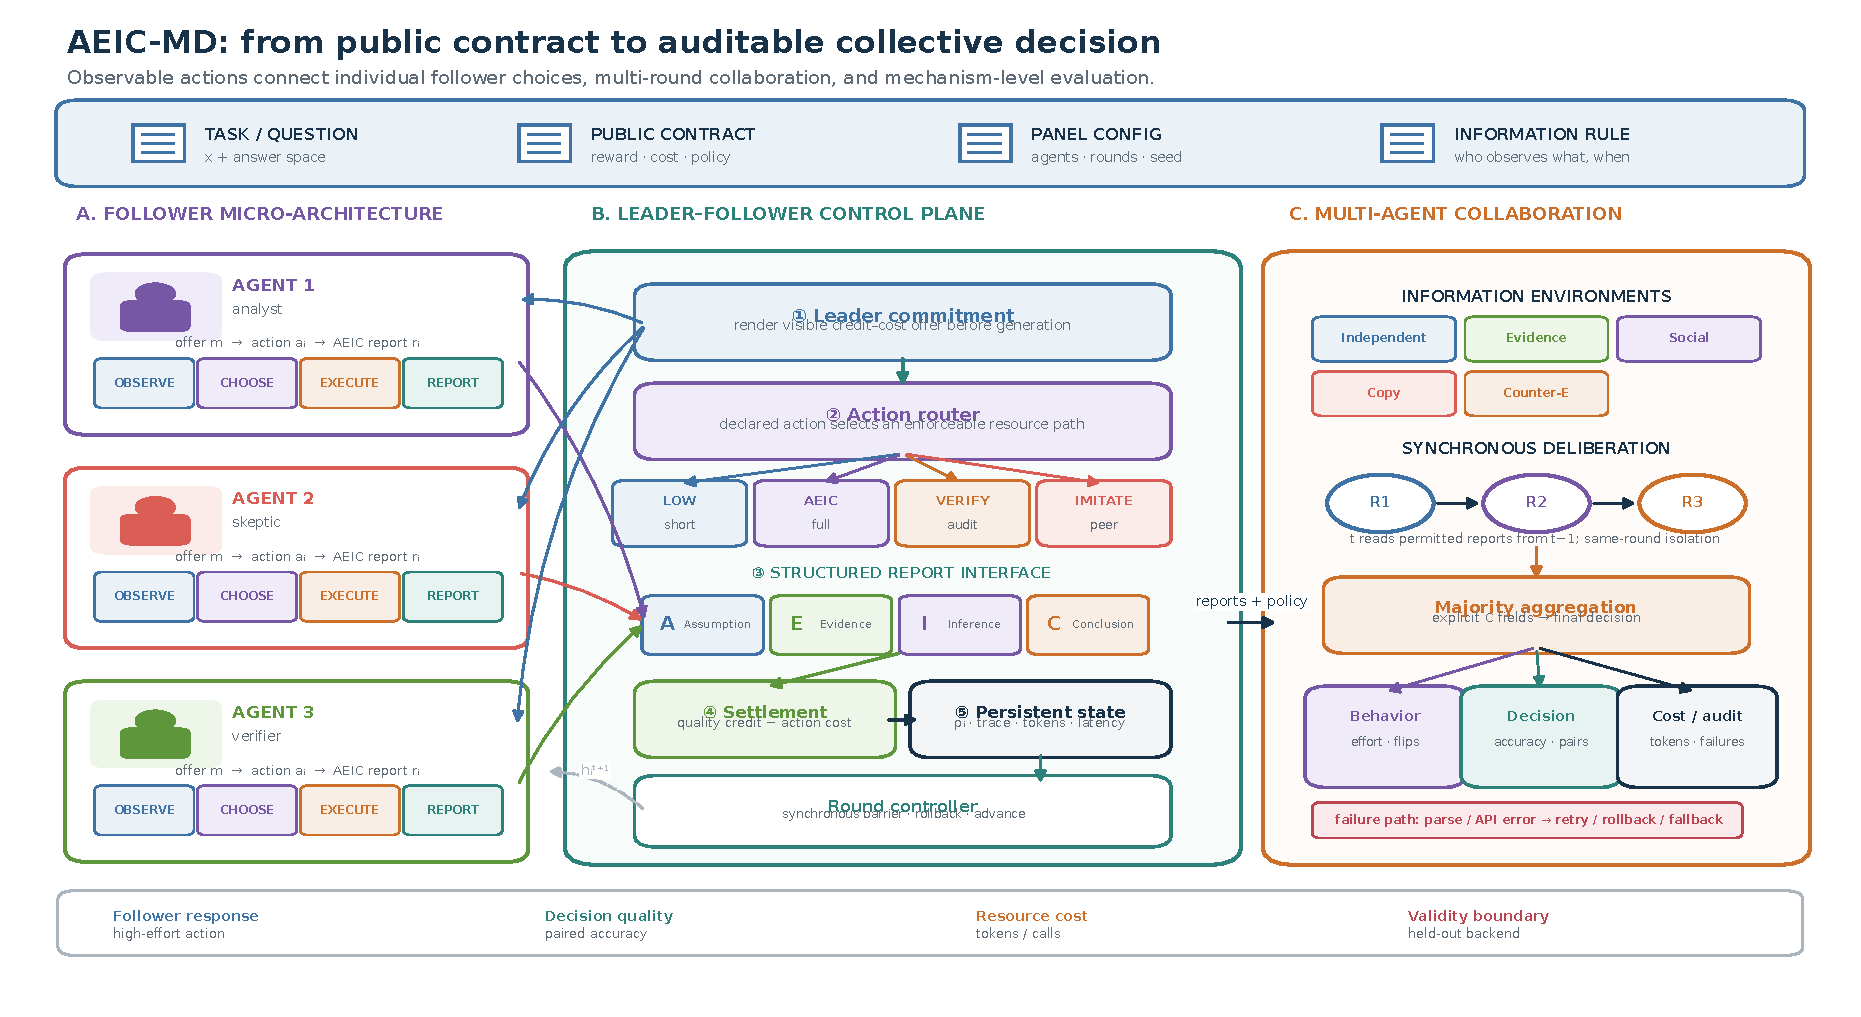
\includegraphics[width=\textwidth]{../figures/fig1_aeic_md_overview_rich.pdf}
\caption{AEIC-MD架构。合同先于资源行动选择，控制器在执行后结算并记录状态。}\label{fig:framework}\end{figure}
